\documentclass{exam}
\newcommand{\splitcell}[2][c]{%
  \begin{tabular}[c]{@{}c@{}}\strut#2\strut\end{tabular}%
}
\usepackage{graphicx} % Required for inserting images
\usepackage{graphics}
\usepackage{float}
\usepackage{tikz}
\usepackage{listings} % Used for the programming coding 
\usepackage{geometry}
\geometry{margin=2cm} %used to fix a warning
\usepackage{xcolor} 
\usepackage{hyperref} %used for the refenrence to a subsection
\usepackage{amsmath}
\usepackage[super]{nth}
\usepackage{svg}

\definecolor{codegreen}{rgb}{0,0.6,0}
\definecolor{codegray}{rgb}{0.5,0.5,0.5}
\definecolor{codepurple}{rgb}{0.58,0,0.82}
\definecolor{backcolour}{rgb}{0.95,0.95,0.92}

\lstdefinestyle{mystyle}{
    backgroundcolor=\color{backcolour},   
    commentstyle=\color{codegreen},
    keywordstyle=\color{magenta},
    numberstyle=\tiny\color{codegray},
    stringstyle=\color{codepurple},
    basicstyle=\ttfamily\footnotesize,
    breakatwhitespace=false,         
    breaklines=true,                 
    captionpos=b,                    
    keepspaces=true,                 
    numbers=none,                    
    numbersep=5pt,                  
    showspaces=false,                
    showstringspaces=false,
    showtabs=false,                  
    tabsize=2
}

\lstset{style=mystyle}



\begin{document}

\newcommand{\Exjobbsnummer}[1]{
	\begin{tikzpicture}[overlay, remember picture]
		\path (current page.north east) ++(-1,-1) node[below left] {{\small #1}};
	\end{tikzpicture}
}

\newcommand{\Examensjobbspoang}[1]{
	\begin{tikzpicture}[overlay, remember picture]
		\path (current page.north east) ++(-1,-1.5) node[below left] {{\normalsize \scshape Examensarbete #1 HP}};
	\end{tikzpicture}
}

\newcommand{\datum}[1]{
	\begin{tikzpicture}[overlay, remember picture]
		\path (current page.north east) ++(-1,-2.0) node[below left] {{\normalsize #1}};
	\end{tikzpicture}}

\newcommand{\storlitentitel}[2]{
\center
\rule[0.2cm]{13cm}{0.1cm}
{ \huge \bfseries #1}\\[0.4cm] % Title of your document
{\Large \slshape #2}\\[0.4cm]
\rule[0.2cm]{13cm}{0.1cm}\\[3cm]

}

\newcommand{\Namn}[2]{
	\begin{minipage}{0.5\textwidth}
		\normalsize
		\centering
		#1 #2\\
	\end{minipage}\\
}



\newcommand{\LoggaSwe}{
	\textsc{\Huge Computer Architecture and \\[0.3cm] Operating Systems}\\[0.3cm]
	
\includegraphics[scale=.06]{graphics/polito_logo_2021_blu.jpg}\\[1.5cm]
}


% -----------------------------------------------
%           start titlepage
%------------------------------------------------
\begin{titlepage}
	\center 



 
	\Exjobbsnummer{Academic Year 2023/2024}	

 
	\LoggaSwe     


 
	\storlitentitel{\\Report}{FreeRTOS: Ingress Firewall}    

    \Namn{Gianfranco} {Trad}
    \Namn{Giorgio} {Fardo}
	\Namn{Luca} {Ponzo}
	\Namn{Michele} {Seira}
        
	\vfill
\end{titlepage}

\pagebreak
\tableofcontents
\pagebreak

\section{Introduction}

In the following report, we will address the \nth{3} and \nth{4} requirements. Having implemented 3 demos related to the \nth{2} requirement, covering both memory management in FreeRTOS and scheduling with preemptive and non-preemptive cases, we have decided to proceed with point 3 by developing an \underline{ingress packet filter}, a basic implementation of a \textbf{firewall}.
\\Specifically we will apply a thorough packet filter by analyzing certain fields, such as IP addresses, ports and protocol, and allowing or denying the entry of each single packet traversing the IP stack of FreeRTOS. In our case the packets are generated with the \textbf{Scapy} tool, which generates packets based on various protocols ( e.g. TCP, UDP, ICMP).
\\The rules are defined as a \textbf{whitelist}, meaning that only those packets that match with one of the rules are allowed. The following snippet represents the rule type we defined. These rules are defined at \textbf{compile-time} by exploiting the \textit{rulegen.py} script that parses \textit{YAML}-like input rules into an array of rules defined in the \textbf{rules.h} header.
\begin{lstlisting}
    typedef struct rule {
      uint32_t src;  // Source IP address in network byte order
      uint32_t dst;  // Destination IP address in network byte order
      uint16_t port_src; // Source port number in network byte order
      uint16_t port_dst; // Destination port number in network byte order
      uint8_t proto; // 2-bit mask representing protocol type
      uint8_t action; //action to do with packets from the source ip 0 >> accept packets 1 >> reject packets
    }Rule;
\end{lstlisting}
Additionally, the Project decisions carried out are easily compatible with a \textbf{blacklist} approach, by just re-defining the \textit{action} field in the rules. This approach was taken in order to enhance the interoperability of our Project also to other use-cases.

\section{Development}

Firstly, by examining the source code of \textbf{FreeRTOS-Plus-TCP}, various files dedicated to packet handling in FreeRTOS can be observed. Through the study of the source code, we have managed to identify the diagram that specifies the flow of all packets arriving to the network interface, followed by their subsequent management through various functions.
More specifically, the packets are processed in the \textbf{FreeRTOS\_IP.c} file, which contains a function named \textbf{prvProcessIPPacket}, that processes the packets at \textit{L3}, defined as follows:

\begin{lstlisting}
   static eFrameProcessingResult_t prvProcessIPPacket( const IPPacket_t * pxIPPacket, NetworkBufferDescriptor_t * const pxNetworkBuffer );
\end{lstlisting}
Which inputs are:
\begin{enumerate}
\item A pointer to the structure representing the packet's IP header:
\begin{lstlisting}
    struct xIP_PACKET
{
    EthernetHeader_t xEthernetHeader;
    IPHeader_t xIPHeader;
}
\end{lstlisting}
\item A pointer to the structure representing the Network\_Buffer:
\begin{lstlisting}
typedef struct xNETWORK_BUFFER
{
    ListItem_t xBufferListItem;                /**< Used to reference the buffer form the free buffer list or a socket. */
    IP_Address_t xIPAddress;                   /**< Source or destination IP address, depending on usage scenario. */
    uint8_t * pucEthernetBuffer;               /**< Pointer to the start of the Ethernet frame. */
    size_t xDataLength;                        /**< Starts by holding the total Ethernet frame length, then the UDP/TCP payload length. */
    struct xNetworkInterface * pxInterface;    /**< The interface on which the packet was received. */
    struct xNetworkEndPoint * pxEndPoint;      /**< The end-point through which this packet shall be sent. */
    uint16_t usPort;                           /**< Source or destination port, depending on usage scenario. */
    uint16_t usBoundPort;                      /**< The port to which a transmitting socket is bound. */
    #if ( ipconfigUSE_LINKED_RX_MESSAGES != 0 )
        struct xNETWORK_BUFFER * pxNextBuffer; /**< Possible optimisation for expert users - requires network driver support. */
    #endif

#define ul_IPAddress     xIPAddress.xIP_IPv4
#define x_IPv6Address    xIPAddress.xIP_IPv6
} NetworkBufferDescriptor_t;
\end{lstlisting}
\end{enumerate}
It is important to note how the decision to insert the firewall at this specific point reduces the \textbf{attack surface} for the attackers. Lastly, checks also on UDP and TCP packets (\textit{L4}) are performed at this level, instead of delaying this checks later on.
\subsubsection*{Packet Flow Graph with the Firewall}
Within this function, two different packet handling methods are distinguished based on the possible types of IP addresses associated with a given packet. However, we will focus exclusively on analyzing \textit{IPv4 packets}.
\begin{figure}[h]
    \centering
    \includesvg[inkscapelatex=false,width=0.70\textwidth]{graphics/callStack.svg}
    \caption{Packet Flow Graph}
    \label{figure1}
\end{figure}
\\The \textbf{firewall} is implemented by the \textit{checkPacketAgainstRules} function that filters the ingress packets by using the predefined rules. The packet filter, was inserted right after Kernel's routine checks on packets such as verifying the correctness of the header length.
The definition of the function is:
\begin{lstlisting}
    uint8_t checkPacketAgainstRules(struct rule ruleset[], int num_rules,const IPHeader_t * pxIPHeader, NetworkBufferDescriptor_t const * pxNetworkBuffer))
\end{lstlisting}
The aforementioned function will return the value \textit{0} when the packet meets one of the defined rules, meaning that it is an allowed packet, whereas, the value 1 when the packet is filtered as ineligible for passage, hence, being a packet that doesn't respect the defined rules.
\\The input parameters of the \textbf{checkPacketAgainstRules} function are:
\begin{enumerate}
\item The structure of the ruleset defined at run-time in the rules.h header.
\item Num\_Rules that defines the number of rules implemented in the whitelist. 
\item Pointer to the structure of the incoming IP packet header that is defined as follow:
\begin{lstlisting}
    struct xIP_HEADER
{
    uint8_t ucVersionHeaderLength;        /**< The version field + internet header length 0 + 1 =  1 */
    uint8_t ucDifferentiatedServicesCode; /**< Differentiated services code point + ECN   1 + 1 =  2 */
    uint16_t usLength;                    /**< Entire Packet size, ex. Ethernet header.   2 + 2 =  4 */
    uint16_t usIdentification;            /**< Identification field                       4 + 2 =  6 */
    uint16_t usFragmentOffset;            /**< Fragment flags and fragment offset         6 + 2 =  8 */
    uint8_t ucTimeToLive;                 /**< Time to live field                         8 + 1 =  9 */
    uint8_t ucProtocol;                   /**< Protocol used in the IP-datagram           9 + 1 = 10 */
    uint16_t usHeaderChecksum;            /**< Checksum of the IP-header                 10 + 2 = 12 */
    uint32_t ulSourceIPAddress;           /**< IP address of the source                  12 + 4 = 16 */
    uint32_t ulDestinationIPAddress;      /**< IP address of the destination             16 + 4 = 20 */
}
\end{lstlisting}
\item The pointer to the structure defined below will be used to check the source and destination ports of the incoming packet for UDP and TCP packets. This parameter is needed in order to perform checks on \textit{L4} information such as the ports, already at this point.
\begin{lstlisting}
    NetworkBufferDescriptor_t const * pxNetworkBuffer
\end{lstlisting}
\end{enumerate}
The function, after taking as input the previously declared values, handles the incoming packet through a switch construct, addressing three different protocol possibilities and in the default case the remaining protocols.
\begin{enumerate}
	\item	\textbf{ipPROTOCOL\_UDP}
	\item	\textbf{ipPROTOCOL\_TCP}
        \item   \textbf{ipPROTOCOL\_ICMP}
	\item	\textbf{default}
\end{enumerate}
In the first case, which deals with \textbf{UDP} packets, the UDP header is extracted and used as input in the following process:
\begin{lstlisting}
    uint8_t checkPacketsWithPorts(struct rule ruleset[], int num_rules, const IPHeader_t * pxIPHeader, uint16_t usSourcePort, uint16_t usDestinationPort)
\end{lstlisting}
It uses the following input parameters:
\begin{enumerate}
\item The predefined ruleset
\item The global constant num\_rules
\item Pointer to the IP packet header
\item Source port of the packet. Extracted from the UDP header from the NetworkBufferDescriptor type passed.
\item Destination port of the packet. Extracted from the UDP header from the NetworkBufferDescriptor type passed.
\end{enumerate}
The check performed on incoming UDP packets is the following one:
\begin{lstlisting}
    for (i = 0; i < num_rules; i++) {
        if(pxIPHeader->ucProtocol==6){
        if (pxIPHeader->ulSourceIPAddress == ruleset[i].src &&
            pxIPHeader->ulDestinationIPAddress == ruleset[i].dst &&
            usSourcePort == ruleset[i].port_src &&
            usDestinationPort == ruleset[i].port_dst &&
            pxIPHeader->ucProtocol == ruleset[i].proto) {
            return ruleset[i].action; // match found execute corresponding action on the packet this can be used both as blakclist and whitelist.
        }
    return 1; // Forbidden packet, hence has to dropped.
\end{lstlisting}
The second case, instead, deals with \textbf{TCP} packets. At the implementation level, a pointer \textbf{pxProtocolHeaders} is extracted using this procedure.
\begin{lstlisting}
    const ProtocolHeaders_t *pxProtocolHeaders = ( ( ProtocolHeaders_t * ) &( pxNetworkBuffer->pucEthernetBuffer[ ipSIZE_OF_ETH_HEADER + uxIPHeaderSizePacket( pxNetworkBuffer ) ] ) );
\end{lstlisting}
Subsequently, this result is used in the \textbf{checkPacketsWithPorts} function (above mentioned), performed the same check performed for UDP packets on ports, addresses and protocol.
\\If the \textbf{checkPacketsWithPorts} function returns the value 1, thus not respecting the firewall rules, the packet is \textbf{not authorized}.\\
Subsequently, for the dropped packets the \textbf{writeToPcap} function is invoked, which takes as input the IP header, the source port, and the destination port extracted from the \textbf{NetworkBufferDescriptor\_t}.
\begin{lstlisting}
    void writeToPcap(const IPHeader_t  * pxIPHeader, uint16_t usSourcePort, uint16_t usDestinationPort)
\end{lstlisting}
This function will write to the standard output, which is then parsed by the \textit{pcap.py} script that parses the log output by recognizing specific keys related to dropped packets. The dropped packets will be transformed in packets representable in \textit{.pcap} format and saved in the \textit{packets.pcap} file.\\
\\The third case, instead, deals with \textbf{ICMP} packets. At the implementation level, a pointer \textbf{pxProtocolHeaders} is extracted using this procedure.
\begin{lstlisting}
    ICMPPacket_t * pxICMPPacket = ( ( ICMPPacket_t * ) pxNetworkBuffer->pucEthernetBuffer );
    IPHeader_t pxIPHeaderofICMPPacket = (IPHeader_t *)& (pxICMPPacket->xIPHeader);
\end{lstlisting}
And the result is used in the function defined below:
\begin{lstlisting}
    uint8_t checkIPs(struct rule ruleset[], int num_rules, const IPHeader_t * pxIPHeader)
\end{lstlisting}
This function verifies the source IP address, the destination IP address, and the protocol, for those packets that do not carry information regarding the ports. If the packet is discarded, the function \textbf{writeToPcap} is invoked with \textbf{usSourcePort} and \textbf{usDestinationPort} statically set to -1, as they are not defined by ICMP protocol\\
\\The default case treats all remaining protocols by performing a check on the addresses and the protocol defined in the rules. Again, the function used is the \textbf{uint8\_t checkIPs} function abovementioned.
\subsection{Ruleset generation}
To generate the rules that we inject statically into the \textbf{rules.h} file a Python script, named \textit{rulegen.py} that translates from \textit{YAML}-like input of the firewall rules to a header file \textit{rules.h} defining an array of rules at compile-time.
\subsection{Packet generation}
The packets sent to the network card were generated via the \textbf{Scapy} module in Python.
\subsection{Pcap Output}
The output in \textit{.pcap} format of the dropped packets by the firewall are generated by the \textit{pcap.py} script.
\pagebreak
\section{Performance Evaluation}
\subsection{Automation}
All the configuration, compiling, linking and running of the \nth{3} and \nth{4} parts were automated by bash scripts, namely the \textit{run\_demo.sh} and the \textit{fireDemoLauncher.sh}.
\begin{itemize}
    \item run\_demo.sh: runs a TCP echo demo to test the TCP stack of the FreeRTOS Kernel.
    \item fireDemoLauncher.sh: 
        \begin{itemize}
            \item Allows to define the firewall rules in YAML format, injects them into a C array of rules defining the firewall via the rulegen.py script.
            \item Starts QEMU and generates 6 packets (2 UDP, 2 TCP, 2 ICMP) via the \textit{Scapy} tool, with 3 of them allowed packets and 3 of them forbidden packets. One allowed packet for each protocol and one forbidden packet for each protocol.
            \item The designed firewall will drop the 3 forbidden packets and produce a log file \textit{out.log} containing information regarding the dropped packets.
            \item The dropped packets' information in the log file will be parsed by the \textit{pcap.py} script which generates a .pcap file containing the packets dropped by the firewall.
        \end{itemize}
    \end{itemize}
\subsection{Firewall Performance}
In the following images, firstly, the packets sent to the network card will be presented. Secondly, the dropped packets by the firewall will be shown.
\subsubsection*{Sent Packets}
\begin{figure}[h]
    \centering
    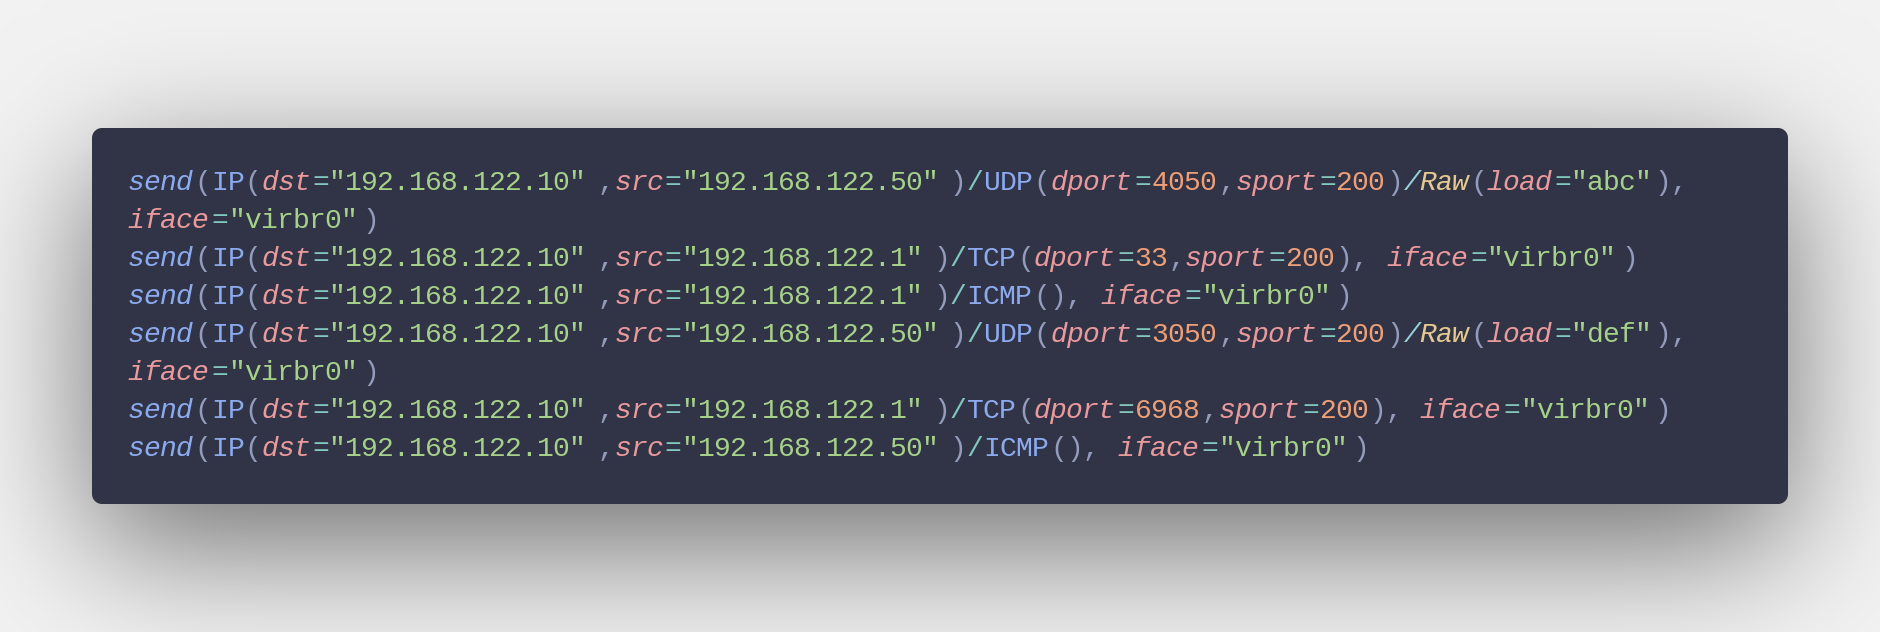
\includegraphics[width=0.90\textwidth]{graphics/scapyRules.png}
    \caption{Packets generated with scapy and sent to the FreeRTOS instance}
\end{figure}
\subsubsection*{Firewall: Dropped Packets}
\begin{figure}[H]
    \centering
    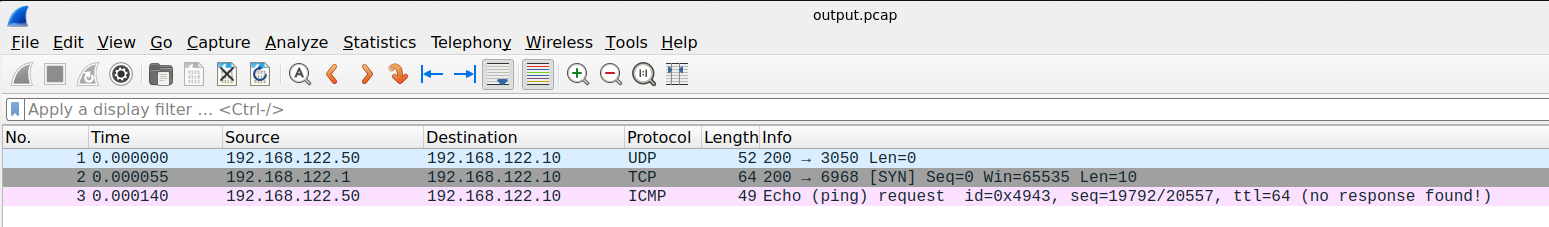
\includegraphics[width=0.9\textwidth]{images/droppedPcap.png}
    \caption{Generated PCAP of the packets dropped by the firewall}
\end{figure}
As the images show the designed firewall is able to \textbf{effectively} filter the non-permitted packets by not allowing them and therefore preventing them from being fully processed by the FreeRTOS Kernel.
\pagebreak
\section{Work In Progress}
As we were dealing with the Project 2 additional features that can be added in the future are:
\begin{itemize}
    \item Intrusion Detection System (IDS) Integration to create a double line of defense.
    \item Support for IPv6 packets.
\end{itemize}
\subsection{IDS Integration}
Regarding the IDS we already performed an initial study and implementation of this possible integration by exploiting the \textbf{Snort} IDS, which is an open-source Intrusion Detection System. The IDS can be placed either before the firewall, if used in blacklist, in order to better set the rules; or after the firewall in order to perform a more thorough checks on the allowed packets.
\begin{figure}[h]
    \centering
    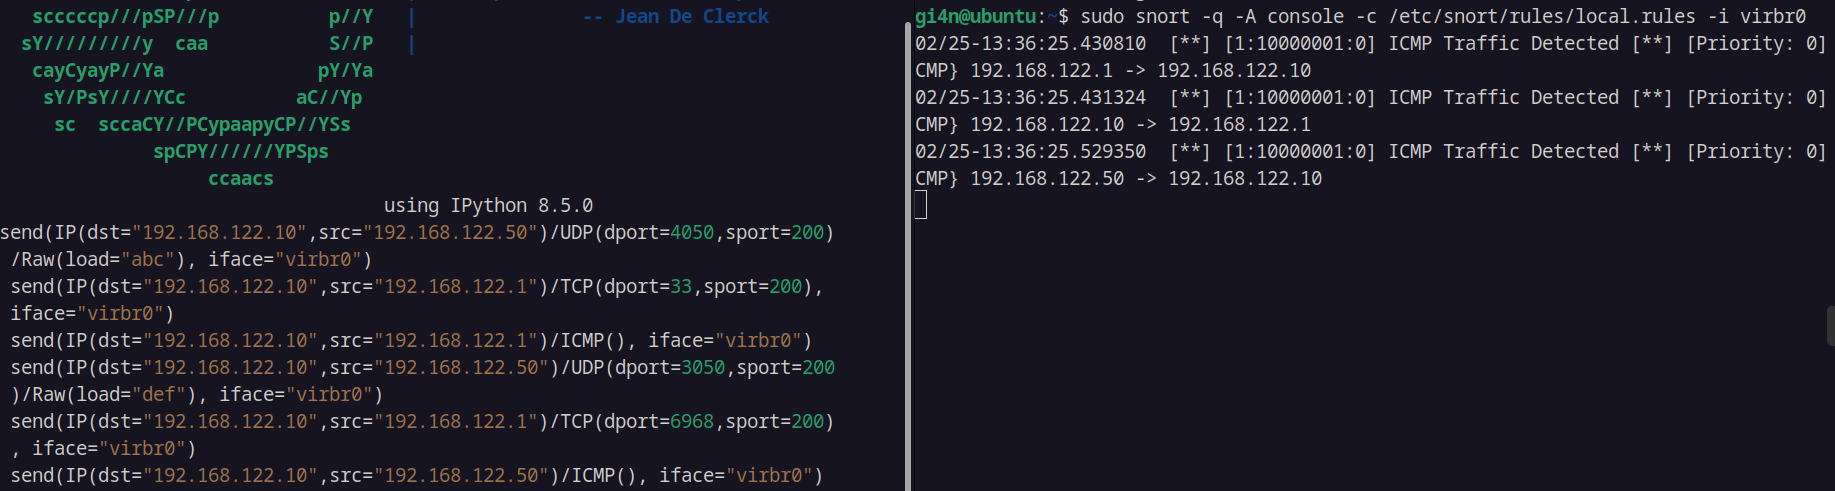
\includegraphics[width=0.9\textwidth]{images/snort.png}
    \caption{Initial PCAP}
\end{figure}
\\For now, we decided to position the IDS before the firewall in order to get more information regarding the Ingress Flow. Additionally, the only rule we have set for now is to produce an alert for incoming and outgoing ICMP packets, which can be exploited to perform some attacks such as ICMP flooding attacks.\\ Of course, more rules can be added. Hence, this is why we inserted this solution still as a \textit{Future Work}.

\end{document}
